% Need to compile under XeTex or XeLaTeX

\documentclass{beamer}

\input{preamble.tex}

\subtitle{第三节:还有幻灯,还有……}

\newcommand{\alice}[1]{\todo[color=green!40]{#1}}
\newcommand{\bob}[1]{\todo[color=purple!40]{#1}}

\begin{document}

%%%%%%%%%%%%%%%%%%%%%%%%%%%%%%%%%%%%%%%%%%%%%%%%%%%%%%%%%%%%%%%%%%%%%%%%%%%%%%%
%%%%%%%%%%%%%%%%%%%%%%%%%%%%%%%%%%%%%%%%%%%%%%%%%%%%%%%%%%%%%%%%%%%%%%%%%%%%%%%
%%%%%%%%%%%%%%%%%%%%%%%%%%%%%%%%%%%%%%%%%%%%%%%%%%%%%%%%%%%%%%%%%%%%%%%%%%%%%%%
\begin{frame}
\titlepage
\end{frame}

%%%%%%%%%%%%%%%%%%%%%%%%%%%%%%%%%%%%%%%%%%%%%%%%%%%%%%%%%%%%%%%%%%%%%%%%%%%%%%%
%%%%%%%%%%%%%%%%%%%%%%%%%%%%%%%%%%%%%%%%%%%%%%%%%%%%%%%%%%%%%%%%%%%%%%%%%%%%%%%
%%%%%%%%%%%%%%%%%%%%%%%%%%%%%%%%%%%%%%%%%%%%%%%%%%%%%%%%%%%%%%%%%%%%%%%%%%%%%%%
%\begin{frame}{Setup}
%\begin{itemize}
%\item Go to this URL in Google Chrome (\emph{not} Internet Explorer) to open
%these slides on your computer in English:
%\vskip 1em
%\begin{center}
%\fbox{\url{http://bit.ly/12WWWqj}}
%\end{center}
%\vskip 1em
%\begin{center}
%\fbox{\href{https://github.com/tanjz12/latex-course/tree/master/zh-cn}{中文版}}
%\end{center}
%\vskip 2em
%\item Here are the slides from the previous tutorial, for reference:
%\begin{center}
%\vskip 1em
%\fbox{\href{https://dl.dropboxusercontent.com/u/31383671/site/latex_course_v2/part1.pdf}{Part 1: The Basics}}
%\vskip 1em
%\fbox{\href{https://dl.dropboxusercontent.com/u/31383671/site/latex_course_v2/part2.pdf}{Part 2: Structured Documents \& More}}
%\end{center}
%\end{itemize}
%\end{frame}

%%%%%%%%%%%%%%%%%%%%%%%%%%%%%%%%%%%%%%%%%%%%%%%%%%%%%%%%%%%%%%%%%%%%%%%%%%%%%%%
%%%%%%%%%%%%%%%%%%%%%%%%%%%%%%%%%%%%%%%%%%%%%%%%%%%%%%%%%%%%%%%%%%%%%%%%%%%%%%%
%%%%%%%%%%%%%%%%%%%%%%%%%%%%%%%%%%%%%%%%%%%%%%%%%%%%%%%%%%%%%%%%%%%%%%%%%%%%%%%
\section{\LaTeX{} 复习}

%%%%%%%%%%%%%%%%%%%%%%%%%%%%%%%%%%%%%%%%%%%%%%%%%%%%%%%%%%%%%%%%%%%%%%%%%%%%%%%
%%%%%%%%%%%%%%%%%%%%%%%%%%%%%%%%%%%%%%%%%%%%%%%%%%%%%%%%%%%%%%%%%%%%%%%%%%%%%%%
%%%%%%%%%%%%%%%%%%%%%%%%%%%%%%%%%%%%%%%%%%%%%%%%%%%%%%%%%%%%%%%%%%%%%%%%%%%%%%%
\begin{frame}[fragile]{\insertsection}
\begin{itemize}
\item 你输入纯文本\texttt{plain text},再用命令 \cmd{commands} 描述其结构、目的和效果。
\item \texttt{latex} 编译器处理命令,生成漂亮排版。
\end{itemize}
\vskip 2ex
\begin{center}
\begin{minted}[frame=single]{latex}
你是\emph{萍,--凭,}--凭什么打我的儿子? 
\end{minted}
\vskip 2ex
\tikz\node[single arrow,fill=lime,font=\ttfamily\bfseries,%
  rotate=270,xshift=-1em]{\ \large{latex}\ \ \ };
\vskip 2ex
\fbox{你是\emph{萍,——凭,}——凭什么打我的儿子?}
\end{center}
\end{frame}

%%%%%%%%%%%%%%%%%%%%%%%%%%%%%%%%%%%%%%%%%%%%%%%%%%%%%%%%%%%%%%%%%%%%%%%%%%%%%%%
%%%%%%%%%%%%%%%%%%%%%%%%%%%%%%%%%%%%%%%%%%%%%%%%%%%%%%%%%%%%%%%%%%%%%%%%%%%%%%%
%%%%%%%%%%%%%%%%%%%%%%%%%%%%%%%%%%%%%%%%%%%%%%%%%%%%%%%%%%%%%%%%%%%%%%%%%%%%%%%
\begin{frame}[fragile]{\insertsection: 命令 \& 参数}
\begin{itemize}
\item 命令开头由\emph{backslash/反斜线} \keystrokebftt{\bs}标识。
\item 有的命令需要参数;参数\emph{argument}放在花括号 \keystrokebftt{\{}
\keystrokebftt{\}}里。
\item 有的命令提供可选参数 \emph{optional arguments}。这些非必需的参数放在方括号\keystrokebftt{[} \keystrokebftt{]}里。
\vskip 2ex
\begin{exampletwouptiny}
\includegraphics[ % 文件名为必须
  width=0.5\textwidth]{gerbil}

\includegraphics[ % 旋转和相对宽度
  width=0.3\textwidth,
  angle=270]{gerbil}
\end{exampletwouptiny}
\end{itemize}

\tiny{图像使用许可:\href{https://pixabay.com/en/animal-apple-attractive-beautiful-1239390/}{CC0}}
\end{frame}

%%%%%%%%%%%%%%%%%%%%%%%%%%%%%%%%%%%%%%%%%%%%%%%%%%%%%%%%%%%%%%%%%%%%%%%%%%%%%%%
%%%%%%%%%%%%%%%%%%%%%%%%%%%%%%%%%%%%%%%%%%%%%%%%%%%%%%%%%%%%%%%%%%%%%%%%%%%%%%%
%%%%%%%%%%%%%%%%%%%%%%%%%%%%%%%%%%%%%%%%%%%%%%%%%%%%%%%%%%%%%%%%%%%%%%%%%%%%%%%
\begin{frame}[fragile]{\insertsection: 情境}
\begin{itemize}
\item 开始 \cmdbs{begin} 和结束 \cmdbs{end} 命令能定义许多情境。

\item \bftt{itemize} 和 \bftt{enumerate} 生成列表。
\vskip 2ex
\begin{exampletwouptiny}
\begin{itemize} % 无序列表
\item[-] 符号自定义
\item[什么] 都可以
\end{itemize}

\begin{enumerate} % 有序列表
\item 没有太大自由
\item 但也有选项 % 宏包和自定义命令
\end{enumerate}

\end{exampletwouptiny}
\end{itemize}
\end{frame}

%%%%%%%%%%%%%%%%%%%%%%%%%%%%%%%%%%%%%%%%%%%%%%%%%%%%%%%%%%%%%%%%%%%%%%%%%%%%%%%
%%%%%%%%%%%%%%%%%%%%%%%%%%%%%%%%%%%%%%%%%%%%%%%%%%%%%%%%%%%%%%%%%%%%%%%%%%%%%%%
%%%%%%%%%%%%%%%%%%%%%%%%%%%%%%%%%%%%%%%%%%%%%%%%%%%%%%%%%%%%%%%%%%%%%%%%%%%%%%%
\begin{frame}[fragile]{\insertsection: Mathematics}
\begin{itemize}
\item 公式 \bftt{equation} 情境生成带编号的数学表达式。
\begin{exampletwouptiny}
\begin{equation}
  \sum_{k=1}^{n} \frac{1}{2^k}
\end{equation}
\end{exampletwouptiny}
\vskip 2ex

\item 用美元符号 \keystrokebftt{\$} 标记行内数学式。\\[1ex]
\begin{exampletwouptiny}
% 纯文本:
令a和b为不等正整数,
再令 c = a - b + 1。

% 经处理:
令$a$和$b$为不等正整数,
再令 $c = a - b + 1$。
\end{exampletwouptiny}
\vskip 2ex
\item \$ 符号必须成对出现——一个标志【表达式】区域开始,另一个表示结束。
\vskip 1em
{\scriptsize 其实 \bftt{\$...\$} 相当于
\cmdbegin{math}\bftt{...}\cmdend{math}.}
\end{itemize}
\end{frame}

%%%%%%%%%%%%%%%%%%%%%%%%%%%%%%%%%%%%%%%%%%%%%%%%%%%%%%%%%%%%%%%%%%%%%%%%%%%%%%%
%%%%%%%%%%%%%%%%%%%%%%%%%%%%%%%%%%%%%%%%%%%%%%%%%%%%%%%%%%%%%%%%%%%%%%%%%%%%%%%
%%%%%%%%%%%%%%%%%%%%%%%%%%%%%%%%%%%%%%%%%%%%%%%%%%%%%%%%%%%%%%%%%%%%%%%%%%%%%%%
\begin{frame}[fragile]{\insertsection: 文档结构}
\begin{itemize}{\small
\item 第一条命令总是 \cmdbs{documentclass} ——文档类型。
\item 把预设的基本信息 (如标题\cmdbs{title} 和作者 \cmdbs{author}) 和需要导入的宏包放在头文件。
\item 全文要显示的部分放在 \cmdbegin{document} 和 \cmdend{document}之间。
\item \cmdbs{maketitle} 命令生成标题(包括作者,日期等) \cmdbs{section} 命令生成章节标题。
}\end{itemize}
\begin{minipage}{0.55\linewidth}
\inputminted[fontsize=\scriptsize,frame=single,resetmargins]{latex}%
  {recap-structure.tex}
\end{minipage}
\begin{minipage}{0.35\linewidth}
% trim: l b r t
\includegraphics[width=\textwidth,clip,trim=1.5in 7in 3in 2in]{recap-structure.pdf}
\end{minipage}
\end{frame}

%%%%%%%%%%%%%%%%%%%%%%%%%%%%%%%%%%%%%%%%%%%%%%%%%%%%%%%%%%%%%%%%%%%%%%%%%%%%%%%
%%%%%%%%%%%%%%%%%%%%%%%%%%%%%%%%%%%%%%%%%%%%%%%%%%%%%%%%%%%%%%%%%%%%%%%%%%%%%%%
%%%%%%%%%%%%%%%%%%%%%%%%%%%%%%%%%%%%%%%%%%%%%%%%%%%%%%%%%%%%%%%%%%%%%%%%%%%%%%%
\begin{frame}[fragile]{\insertsection: 练习}

\begin{enumerate}
\item 这里有一篇小文章\footnote{由 \url{http://www.cgd.ucar.edu/cms/agu/scientific_talk.html} 删改}
\begin{center}
\fbox{\href{\wlnewdoc{recap-exercise.tex}}{%
点此在\wllogo{}中打开该文档}}
\end{center}
\vskip 2ex
\item 添加一些\LaTeX{} 命令把它变成这样
\begin{center}
\fbox{\href{\fileuri/recap-exercise-solution.pdf} ,需先将它用反斜线(\cmdbs{\%}) 进行 \emph{强制转换/escape} 
\item 打方程式时,用 \cmdbs{frac} 表示分数,用 \cmdbs{left(} and \cmdbs{right)} 命令打出可自动调整大小的括弧。
\end{itemize}
\end{block}
\end{frame}

%%%%%%%%%%%%%%%%%%%%%%%%%%%%%%%%%%%%%%%%%%%%%%%%%%%%%%%%%%%%%%%%%%%%%%%%%%%%%%%
%%%%%%%%%%%%%%%%%%%%%%%%%%%%%%%%%%%%%%%%%%%%%%%%%%%%%%%%%%%%%%%%%%%%%%%%%%%%%%%
%%%%%%%%%%%%%%%%%%%%%%%%%%%%%%%%%%%%%%%%%%%%%%%%%%%%%%%%%%%%%%%%%%%%%%%%%%%%%%%
\section{\small{用} \protect\bftt{beamer}\small{做}演讲}

%%%%%%%%%%%%%%%%%%%%%%%%%%%%%%%%%%%%%%%%%%%%%%%%%%%%%%%%%%%%%%%%%%%%%%%%%%%%%%%
%%%%%%%%%%%%%%%%%%%%%%%%%%%%%%%%%%%%%%%%%%%%%%%%%%%%%%%%%%%%%%%%%%%%%%%%%%%%%%%
%%%%%%%%%%%%%%%%%%%%%%%%%%%%%%%%%%%%%%%%%%%%%%%%%%%%%%%%%%%%%%%%%%%%%%%%%%%%%%%
\begin{frame}[fragile]{\insertsection}
\begin{itemize}
\item Beamer是一个用\LaTeX{}做幻灯的宏包。
\item 它提供 \bftt{beamer} 文件类型
\item 每个 \bftt{frame} 情境对应一张幻灯
\end{itemize}
\begin{minipage}{0.55\linewidth}
\inputminted[fontsize=\scriptsize,frame=single,resetmargins]{latex}%
  {beamer-minimal.tex}
\end{minipage}
\begin{minipage}{0.35\linewidth}
% trim: l b r t
\includegraphics[width=\textwidth,clip,trim=1in 1in 1in 1in]{beamer-minimal.pdf}
\end{minipage}
\end{frame}

%%%%%%%%%%%%%%%%%%%%%%%%%%%%%%%%%%%%%%%%%%%%%%%%%%%%%%%%%%%%%%%%%%%%%%%%%%%%%%%
%%%%%%%%%%%%%%%%%%%%%%%%%%%%%%%%%%%%%%%%%%%%%%%%%%%%%%%%%%%%%%%%%%%%%%%%%%%%%%%
%%%%%%%%%%%%%%%%%%%%%%%%%%%%%%%%%%%%%%%%%%%%%%%%%%%%%%%%%%%%%%%%%%%%%%%%%%%%%%%
\begin{frame}[fragile]{\insertsection: 跟着学}

\begin{itemize}
\item 在学习之后的幻灯片时,请你也动手试一试。可以本地安装\LaTeX{},也可以在\wllogo{}中打开文档。
\end{itemize}
\vskip 2ex
\begin{center}
\fbox{\href{\wlnewdoc{beamer-minimal.tex}}{%
点此打开 \wllogo{} 示例幻灯片}}
\end{center}
\end{frame}

%%%%%%%%%%%%%%%%%%%%%%%%%%%%%%%%%%%%%%%%%%%%%%%%%%%%%%%%%%%%%%%%%%%%%%%%%%%%%%%
%%%%%%%%%%%%%%%%%%%%%%%%%%%%%%%%%%%%%%%%%%%%%%%%%%%%%%%%%%%%%%%%%%%%%%%%%%%%%%%
%%%%%%%%%%%%%%%%%%%%%%%%%%%%%%%%%%%%%%%%%%%%%%%%%%%%%%%%%%%%%%%%%%%%%%%%%%%%%%%
\begin{frame}[fragile]
\frametitle{\insertsection: 幻灯页}
\begin{itemize}
\item 用 \cmdbs{frametitle} 设置幻灯页标题。
\item 再添加内容。
\item 本页面源码在这里……
\vskip 2ex
\inputminted[fontsize=\scriptsize,frame=single,resetmargins]{latex}%
  {beamer-frame.tex}
\end{itemize}
\end{frame}

%%%%%%%%%%%%%%%%%%%%%%%%%%%%%%%%%%%%%%%%%%%%%%%%%%%%%%%%%%%%%%%%%%%%%%%%%%%%%%%
%%%%%%%%%%%%%%%%%%%%%%%%%%%%%%%%%%%%%%%%%%%%%%%%%%%%%%%%%%%%%%%%%%%%%%%%%%%%%%%
%%%%%%%%%%%%%%%%%%%%%%%%%%%%%%%%%%%%%%%%%%%%%%%%%%%%%%%%%%%%%%%%%%%%%%%%%%%%%%%
\begin{frame}[fragile]{\insertsection: 章节}
\begin{itemize}
\item 你可以用 \cmdbs{section} 组织你的幻灯片 \bftt{frame};
\bftt{beamer} 会自动提取信息组成目录.
\item 用 \cmdbs{tableofcontents} 生成目录。以下是这部幻灯片的目录。在方括号内输入\bftt{currentsection} 选项可以高亮目前章节。
\vskip 2ex
\begin{exampletwouptiny}
\tableofcontents[currentsection]
\end{exampletwouptiny}
\end{itemize}
\end{frame}

%%%%%%%%%%%%%%%%%%%%%%%%%%%%%%%%%%%%%%%%%%%%%%%%%%%%%%%%%%%%%%%%%%%%%%%%%%%%%%%
%%%%%%%%%%%%%%%%%%%%%%%%%%%%%%%%%%%%%%%%%%%%%%%%%%%%%%%%%%%%%%%%%%%%%%%%%%%%%%%
%%%%%%%%%%%%%%%%%%%%%%%%%%%%%%%%%%%%%%%%%%%%%%%%%%%%%%%%%%%%%%%%%%%%%%%%%%%%%%%
\begin{frame}[fragile]{\insertsection: 多列排版}
\begin{columns}
\begin{column}{0.4\textwidth}
\begin{itemize}
\item 用\bftt{columns} 和 \bftt{column} 情境分栏。
\item 每个 \bftt{column} 的宽度由参数决定。
\item 参见 \bftt{multicol} 宏包(含自动分栏效果)。
\end{itemize}
\end{column}
\begin{column}{0.6\textwidth}
\begin{minted}[fontsize=\scriptsize,frame=single]{latex}
\begin{columns}
  \begin{column}{0.4\textwidth}
    \begin{itemize}
    \item 用\bftt{columns} 和 \bftt{column} ...
    \item 每个 \bftt{column} 的宽度 ...
    \item 参见 \bftt{multicol} 宏包 ...
    \end{itemize}
  \end{column}
  \begin{column}{0.6\textwidth}
    % second column
  \end{column}
\end{columns}
\end{minted}
\end{column}
\end{columns}
\end{frame}

%%%%%%%%%%%%%%%%%%%%%%%%%%%%%%%%%%%%%%%%%%%%%%%%%%%%%%%%%%%%%%%%%%%%%%%%%%%%%%%
%%%%%%%%%%%%%%%%%%%%%%%%%%%%%%%%%%%%%%%%%%%%%%%%%%%%%%%%%%%%%%%%%%%%%%%%%%%%%%%
%%%%%%%%%%%%%%%%%%%%%%%%%%%%%%%%%%%%%%%%%%%%%%%%%%%%%%%%%%%%%%%%%%%%%%%%%%%%%%%
\begin{frame}[fragile]{\insertsection: 高亮}
\begin{itemize}

\item 用 \cmdbs{emph} 或 \cmdbs{alert} 高亮:
\vskip 1ex
\begin{exampletwouptiny}
我应该 \emph{强调} 这个 \alert{重} 点。
\end{exampletwouptiny}
\vskip 1ex

\item 你想选用粗体和花体也可以:
\vskip 1ex
\begin{exampletwouptiny}
\textbf{粗体}字。
\textit{花体}字。
\end{exampletwouptiny}
\vskip 1ex

\item 或改变颜色 (按AmE美式拼Color):
\vskip 1ex
\begin{exampletwouptiny}
红灯\textcolor{red}{停},
绿灯\textcolor{green}{行}。
\end{exampletwouptiny}
\vskip 1ex
\item 详阅 \url{http://www.math.umbc.edu/~rouben/beamer/quickstart-Z-H-25.html}
中其他颜色 \& 自定义颜色。
\end{itemize}
\end{frame}

%%%%%%%%%%%%%%%%%%%%%%%%%%%%%%%%%%%%%%%%%%%%%%%%%%%%%%%%%%%%%%%%%%%%%%%%%%%%%%%
%%%%%%%%%%%%%%%%%%%%%%%%%%%%%%%%%%%%%%%%%%%%%%%%%%%%%%%%%%%%%%%%%%%%%%%%%%%%%%%
%%%%%%%%%%%%%%%%%%%%%%%%%%%%%%%%%%%%%%%%%%%%%%%%%%%%%%%%%%%%%%%%%%%%%%%%%%%%%%%
\begin{frame}[fragile]{\insertsection: 图象}
\begin{itemize}
\item 用 \bftt{graphicx} 宏包的 \cmdbs{includegraphics} 命令。
\item \bftt{beamer} 中的 \bftt{figure} 情境自动居中。
\vskip 2ex
\begin{exampletwouptiny}
\begin{figure}
\includegraphics[
  width=0.5\textwidth]{gerbil}
\end{figure}
\end{exampletwouptiny}
\end{itemize}

\tiny{图像使用许可:\href{https://pixabay.com/en/animal-apple-attractive-beautiful-1239390/}{CC0}}
\end{frame}

%%%%%%%%%%%%%%%%%%%%%%%%%%%%%%%%%%%%%%%%%%%%%%%%%%%%%%%%%%%%%%%%%%%%%%%%%%%%%%%
%%%%%%%%%%%%%%%%%%%%%%%%%%%%%%%%%%%%%%%%%%%%%%%%%%%%%%%%%%%%%%%%%%%%%%%%%%%%%%%
%%%%%%%%%%%%%%%%%%%%%%%%%%%%%%%%%%%%%%%%%%%%%%%%%%%%%%%%%%%%%%%%%%%%%%%%%%%%%%%
\begin{frame}[fragile]{\insertsection:制表}
\begin{itemize}
\item \LaTeX{} 制表,习惯了其实很方便。
\item 用 \bftt{tabularx} 宏包的 \bftt{tabular}表格情境。 
\item 花括号里是各栏对齐方式——\textbf{l}eft左对齐, \textbf{r}ight右对齐, \textbf{r}ight右对齐.
\begin{exampletwouptiny}
\begin{tabular}{lrr}
物品   & 数量 & 单价 \$ \\
冬瓜   & 1   & 199.99  \\
南瓜   & 2   & 399.99  \\
西瓜   & 3   & 19.99   \\
\end{tabular}
\end{exampletwouptiny}
\item 这部分也能设置纵向分割线; \cmdbs{hline} 生成横向分割线。
\begin{exampletwouptiny}
\begin{tabular}{|l|r|r|} \hline
物品   & 数量 & 单价 \$ \\\hline
冬瓜   & 1   & 199.99  \\
南瓜   & 2   & 399.99  \\
西瓜   & 3   & 19.99   \\\hline
\end{tabular}
\end{exampletwouptiny}
\item 用and符号 \keystrokebftt{\&} 分栏,双反斜线 \keystrokebftt{\bs}\keystrokebftt{\bs} 换行 (和第一部分 \bftt{align*} 情境中格式一样).
\end{itemize}
\end{frame}

%%%%%%%%%%%%%%%%%%%%%%%%%%%%%%%%%%%%%%%%%%%%%%%%%%%%%%%%%%%%%%%%%%%%%%%%%%%%%%%
%%%%%%%%%%%%%%%%%%%%%%%%%%%%%%%%%%%%%%%%%%%%%%%%%%%%%%%%%%%%%%%%%%%%%%%%%%%%%%%
%%%%%%%%%%%%%%%%%%%%%%%%%%%%%%%%%%%%%%%%%%%%%%%%%%%%%%%%%%%%%%%%%%%%%%%%%%%%%%%
\begin{frame}[fragile]{\insertsection: 区块}
\begin{itemize}
\item \bftt{block} 情境可创建带标题的区块。
\begin{exampletwouptiny}
\begin{block}{趣闻}
这里有概要
\end{block}

\begin{alertblock}{悚闻}
标题党的概要
\end{alertblock}
\end{exampletwouptiny}

\item 区块具体格式取决于主题\ldots
\end{itemize}
\end{frame}

%%%%%%%%%%%%%%%%%%%%%%%%%%%%%%%%%%%%%%%%%%%%%%%%%%%%%%%%%%%%%%%%%%%%%%%%%%%%%%%
%%%%%%%%%%%%%%%%%%%%%%%%%%%%%%%%%%%%%%%%%%%%%%%%%%%%%%%%%%%%%%%%%%%%%%%%%%%%%%%
%%%%%%%%%%%%%%%%%%%%%%%%%%%%%%%%%%%%%%%%%%%%%%%%%%%%%%%%%%%%%%%%%%%%%%%%%%%%%%%
\begin{frame}[fragile]
\frametitle{\insertsection: 主题}
\begin{itemize}
\item 用主题整体调整外观
\item 这里收集了各种主题\url{http://deic.uab.es/~iblanes/beamer_gallery/index_by_theme.html}。
\end{itemize}
\begin{minipage}{0.55\linewidth}
\inputminted[fontsize=\scriptsize,frame=single,resetmargins]{latex}%
  {beamer-theme.tex}
\end{minipage}
\begin{minipage}{0.35\linewidth}
% trim: l b r t
\includegraphics[width=\textwidth]{beamer-theme.pdf}
\end{minipage}
\end{frame}

%%%%%%%%%%%%%%%%%%%%%%%%%%%%%%%%%%%%%%%%%%%%%%%%%%%%%%%%%%%%%%%%%%%%%%%%%%%%%%%
%%%%%%%%%%%%%%%%%%%%%%%%%%%%%%%%%%%%%%%%%%%%%%%%%%%%%%%%%%%%%%%%%%%%%%%%%%%%%%%
%%%%%%%%%%%%%%%%%%%%%%%%%%%%%%%%%%%%%%%%%%%%%%%%%%%%%%%%%%%%%%%%%%%%%%%%%%%%%%%
\begin{frame}[fragile]{\insertsection: 动画}
\begin{itemize}
\item 一个\bftt{frame} 可能对应好几张幻灯片
\item 只有\cmdbs{pause} 之上部分会显示。
\vskip 2ex
\begin{exampletwouptinynoframe}
\begin{itemize}
\item 有没有感觉到
\pause \item 悬念?
\end{itemize}
\end{exampletwouptinynoframe}
\vskip 2ex
\item \bftt{beamer}还有很多动画效果;参见 \cmdbs{only}, \cmdbs{alt}, 和 \cmdbs{uncover} 等命令。
\end{itemize}
\end{frame}

%%%%%%%%%%%%%%%%%%%%%%%%%%%%%%%%%%%%%%%%%%%%%%%%%%%%%%%%%%%%%%%%%%%%%%%%%%%%%%%
%%%%%%%%%%%%%%%%%%%%%%%%%%%%%%%%%%%%%%%%%%%%%%%%%%%%%%%%%%%%%%%%%%%%%%%%%%%%%%%
%%%%%%%%%%%%%%%%%%%%%%%%%%%%%%%%%%%%%%%%%%%%%%%%%%%%%%%%%%%%%%%%%%%%%%%%%%%%%%%
\begin{frame}[fragile]{\insertsection: 练习}

英文版练习取自 Peter Norvig 的葛底斯堡演讲幻灯片;中文版是由尚书·牧野改编。试试自己用\bftt{beamer}做这个幻灯片!\footnote{\url{http://norvig.com/Gettysburg}}

\begin{enumerate}
\item 在 \wllogo{} 中打开练习源码:
\begin{center}
\fbox{\href{\wlnewdoc{beamer-exercise.tex}}{%
点此在 \wllogo{}中打开文档}}
\end{center}
\vskip 2ex
\item 你可以在幻灯中使用这幅图;经 files 菜单可上传至\wllogo{}。
\begin{center}
\fbox{\href{\fileuri/Spline-1.png?dl=1}{点此下载}}
\end{center}
\vskip 2ex
\item 添加 \LaTeX{} 命令至以下效果:
\begin{center}
\fbox{\href{\fileuri/beamer-exercise-solution.pdf}{%
点此打开示例}}
\end{center}
\end{enumerate}
\end{frame}

%%%%%%%%%%%%%%%%%%%%%%%%%%%%%%%%%%%%%%%%%%%%%%%%%%%%%%%%%%%%%%%%%%%%%%%%%%%%%%%
%%%%%%%%%%%%%%%%%%%%%%%%%%%%%%%%%%%%%%%%%%%%%%%%%%%%%%%%%%%%%%%%%%%%%%%%%%%%%%%
%%%%%%%%%%%%%%%%%%%%%%%%%%%%%%%%%%%%%%%%%%%%%%%%%%%%%%%%%%%%%%%%%%%%%%%%%%%%%%%
\section{\small{用} \protect\tikzname 绘图}

%%%%%%%%%%%%%%%%%%%%%%%%%%%%%%%%%%%%%%%%%%%%%%%%%%%%%%%%%%%%%%%%%%%%%%%%%%%%%%%
%%%%%%%%%%%%%%%%%%%%%%%%%%%%%%%%%%%%%%%%%%%%%%%%%%%%%%%%%%%%%%%%%%%%%%%%%%%%%%%
%%%%%%%%%%%%%%%%%%%%%%%%%%%%%%%%%%%%%%%%%%%%%%%%%%%%%%%%%%%%%%%%%%%%%%%%%%%%%%%
\begin{frame}[fragile]{\insertsection}
\begin{itemize}
\item \tikzname{} 是 \LaTeX 中的一个绘图宏包。
\item 它借 \LaTeX{} 语法实现强大的绘图功能。几行代码就能画出相当复杂的图形。
\begin{figure}
\href{http://www.texample.net/tikz/examples/rotated-triangle/}{%
  \includegraphics[width=0.35\textwidth]{rotated-triangle}}
\end{figure}
\item 我们从简单图形开始。在这里画条线
\tikzname:
\vskip 1ex
\begin{exampletwouptiny}
\begin{tikzpicture}
\draw (0,0) -- (1,1); % 一条线
\end{tikzpicture}
\end{exampletwouptiny}
\end{itemize}
\end{frame}

%%%%%%%%%%%%%%%%%%%%%%%%%%%%%%%%%%%%%%%%%%%%%%%%%%%%%%%%%%%%%%%%%%%%%%%%%%%%%%%
%%%%%%%%%%%%%%%%%%%%%%%%%%%%%%%%%%%%%%%%%%%%%%%%%%%%%%%%%%%%%%%%%%%%%%%%%%%%%%%
%%%%%%%%%%%%%%%%%%%%%%%%%%%%%%%%%%%%%%%%%%%%%%%%%%%%%%%%%%%%%%%%%%%%%%%%%%%%%%%
\begin{frame}[fragile]{\insertsection: 坐标}
\begin{itemize}
\item 坐标默认以厘米为单位
\begin{figure}
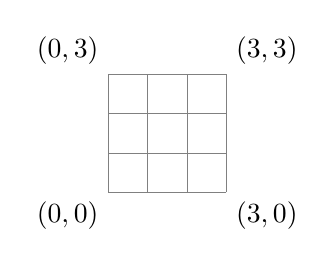
\begin{tikzpicture}[scale=0.5]
\draw[help lines] (0,0) grid (3,3);
\node[below left] at (0,0) {$(0,0)$};
\node[below right] at (3,0) {$(3,0)$};
\node[above right] at (3,3) {$(3,3)$};
\node[above left] at (0,3) {$(0,3)$};
\end{tikzpicture}
\end{figure}
\item 有时你也需要画格,比如 \tikzname :
\vskip 1ex
\begin{exampletwouptiny}

\begin{tikzpicture}
\draw[help lines] (0,0) grid (3,3);
\end{tikzpicture}
\end{exampletwouptiny}
\end{itemize}
\end{frame}

%%%%%%%%%%%%%%%%%%%%%%%%%%%%%%%%%%%%%%%%%%%%%%%%%%%%%%%%%%%%%%%%%%%%%%%%%%%%%%%
%%%%%%%%%%%%%%%%%%%%%%%%%%%%%%%%%%%%%%%%%%%%%%%%%%%%%%%%%%%%%%%%%%%%%%%%%%%%%%%
%%%%%%%%%%%%%%%%%%%%%%%%%%%%%%%%%%%%%%%%%%%%%%%%%%%%%%%%%%%%%%%%%%%%%%%%%%%%%%%
\begin{frame}[fragile]{\insertsection: 线和箭头}
\begin{itemize}
\item \cmdbs{draw} 命令的参数控制线型和箭头。
\item 用\emph{英文分号}\keystrokebftt{;} 结束每个 \cmdbs{draw} 命令
\vskip 1ex
\begin{exampletwouptiny}
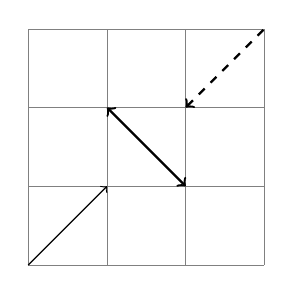
\begin{tikzpicture}
\draw[help lines] (0,0) grid (3,3);
\draw[->] (0,0) -- (1,1);
\draw[<->, thick] (2,1) -- (1,2);
\draw[<-, thick, dashed] (2,2)--(3,3);
\end{tikzpicture}
\end{exampletwouptiny}
\end{itemize}
\end{frame}

%%%%%%%%%%%%%%%%%%%%%%%%%%%%%%%%%%%%%%%%%%%%%%%%%%%%%%%%%%%%%%%%%%%%%%%%%%%%%%%
%%%%%%%%%%%%%%%%%%%%%%%%%%%%%%%%%%%%%%%%%%%%%%%%%%%%%%%%%%%%%%%%%%%%%%%%%%%%%%%
%%%%%%%%%%%%%%%%%%%%%%%%%%%%%%%%%%%%%%%%%%%%%%%%%%%%%%%%%%%%%%%%%%%%%%%%%%%%%%%
\begin{frame}[fragile]{\insertsection: 折线}
\begin{itemize}
\item 你可以用几个点组合线段,形成一条折线
\item 只有整组线段头尾才有箭头
\vskip 1ex
\begin{exampletwouptiny}
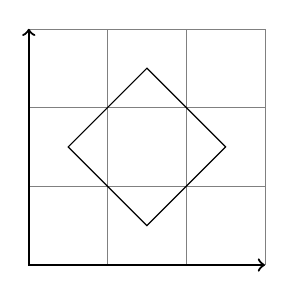
\begin{tikzpicture}
\draw[help lines] (0,0) grid (3,3);
% 坐标轴:
\draw[<->, thick] (0,3)--(0,0)--(3,0);
% 斜放时称diamond,亦指一般菱形:
\draw (1.5,0.5) -- (2.5,1.5) -- 
      (1.5,2.5) -- (0.5,1.5) --
      cycle; % 表示折线结束
\end{tikzpicture}
\end{exampletwouptiny}
\end{itemize}
\end{frame}

%%%%%%%%%%%%%%%%%%%%%%%%%%%%%%%%%%%%%%%%%%%%%%%%%%%%%%%%%%%%%%%%%%%%%%%%%%%%%%%
%%%%%%%%%%%%%%%%%%%%%%%%%%%%%%%%%%%%%%%%%%%%%%%%%%%%%%%%%%%%%%%%%%%%%%%%%%%%%%%
%%%%%%%%%%%%%%%%%%%%%%%%%%%%%%%%%%%%%%%%%%%%%%%%%%%%%%%%%%%%%%%%%%%%%%%%%%%%%%%
\begin{frame}[fragile]{\insertsection: 颜色}
\begin{itemize}
\item \cmdbs{draw} 命令的参数也控制颜色。
\vskip 1ex
\begin{exampletwouptiny}
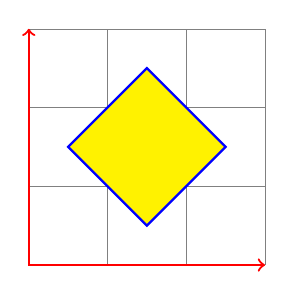
\begin{tikzpicture}
\draw[help lines] (0,0) grid (3,3);
% 坐标轴:
\draw[<->, thick, red]
  (0,3)--(0,0)--(3,0); 
% diamond
\draw[thick, blue, fill=yellow]
  (1.5,0.5) -- (2.5,1.5) -- 
  (1.5,2.5) -- (0.5,1.5) --
  cycle;
\end{tikzpicture}
\end{exampletwouptiny}
\end{itemize}
\end{frame}

%%%%%%%%%%%%%%%%%%%%%%%%%%%%%%%%%%%%%%%%%%%%%%%%%%%%%%%%%%%%%%%%%%%%%%%%%%%%%%%
%%%%%%%%%%%%%%%%%%%%%%%%%%%%%%%%%%%%%%%%%%%%%%%%%%%%%%%%%%%%%%%%%%%%%%%%%%%%%%%
%%%%%%%%%%%%%%%%%%%%%%%%%%%%%%%%%%%%%%%%%%%%%%%%%%%%%%%%%%%%%%%%%%%%%%%%%%%%%%%
\begin{frame}[fragile]{\insertsection: Shapes}
\begin{itemize}
\item \tikzname{} 也内置了简单图形的命令。
\vskip 1ex
\begin{exampletwouptiny}
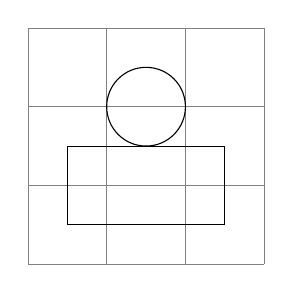
\begin{tikzpicture}
\draw[help lines] (0,0) grid (3,3);
\draw (1.5,2.0) circle (0.5);
\draw (0.5,0.5) rectangle (2.5,1.5);
\end{tikzpicture}
\end{exampletwouptiny}
\end{itemize}
\end{frame}

%%%%%%%%%%%%%%%%%%%%%%%%%%%%%%%%%%%%%%%%%%%%%%%%%%%%%%%%%%%%%%%%%%%%%%%%%%%%%%%
%%%%%%%%%%%%%%%%%%%%%%%%%%%%%%%%%%%%%%%%%%%%%%%%%%%%%%%%%%%%%%%%%%%%%%%%%%%%%%%
%%%%%%%%%%%%%%%%%%%%%%%%%%%%%%%%%%%%%%%%%%%%%%%%%%%%%%%%%%%%%%%%%%%%%%%%%%%%%%%
\begin{frame}[fragile]{\insertsection: 节点 \& 标签}
\begin{itemize}
\item 用 \bftt{node} 在 \tikzname{} 图纸上作注(含数学式)。
\item 比如说坐标可放在 \bftt{node} 中。
\vskip 1ex
\begin{exampletwouptiny}
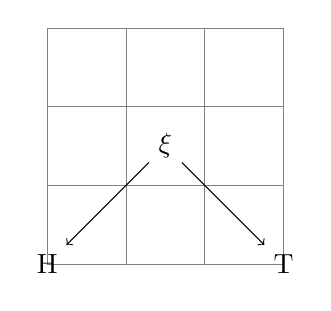
\begin{tikzpicture}
\draw[help lines] (0,0) grid (3,3);
\node (h) at (0,0) {H};
\node (x) at (1.5,1.5) {$\xi$};
\node (t) at (3,0) {T};
\draw[->] (x) -- (h);
\draw[->] (x) -- (t);
\end{tikzpicture}
\end{exampletwouptiny}
\end{itemize}
\end{frame}

%%%%%%%%%%%%%%%%%%%%%%%%%%%%%%%%%%%%%%%%%%%%%%%%%%%%%%%%%%%%%%%%%%%%%%%%%%%%%%%
%%%%%%%%%%%%%%%%%%%%%%%%%%%%%%%%%%%%%%%%%%%%%%%%%%%%%%%%%%%%%%%%%%%%%%%%%%%%%%%
%%%%%%%%%%%%%%%%%%%%%%%%%%%%%%%%%%%%%%%%%%%%%%%%%%%%%%%%%%%%%%%%%%%%%%%%%%%%%%%
\begin{frame}[fragile]{\insertsection: 函数}
\begin{itemize}
\item 你甚至可以绘制简单函数
\vskip 1ex
\begin{exampletwouptiny}
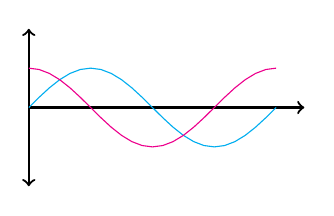
\begin{tikzpicture}[scale=0.5]
% y 轴:
\draw[<->, thick] (0,2) -- (0,-2);
% x 轴:
\draw[ ->, thick] (0,0) -- (7, 0); 
% curves
\draw[cyan,domain=0:2*pi]
  plot (\x, {sin(\x r)});
\draw[magenta,domain=0:2*pi]
  plot (\x, {cos(\x r)});
\end{tikzpicture}
\end{exampletwouptiny}
\end{itemize}
\end{frame}

%%%%%%%%%%%%%%%%%%%%%%%%%%%%%%%%%%%%%%%%%%%%%%%%%%%%%%%%%%%%%%%%%%%%%%%%%%%%%%%
%%%%%%%%%%%%%%%%%%%%%%%%%%%%%%%%%%%%%%%%%%%%%%%%%%%%%%%%%%%%%%%%%%%%%%%%%%%%%%%
%%%%%%%%%%%%%%%%%%%%%%%%%%%%%%%%%%%%%%%%%%%%%%%%%%%%%%%%%%%%%%%%%%%%%%%%%%%%%%%
\begin{frame}[fragile]{\insertsection: 例子}
\begin{itemize}
\item 参见 \fbox{\href{http://texample.net/tikz/}{\TeX{}ample.net}} 中 \tikzname{} 示例:
\end{itemize}
\begin{figure}
\href{http://texample.net/tikz/examples/escher-brick-penrose-triangle/}{%
  \includegraphics[width=0.3\textwidth]{escher-brick-penrose-triangle}}
\href{http://texample.net/tikz/examples/computer-science-mindmap/}{%
  \includegraphics[width=0.3\textwidth]{computer-science-mindmap}}
\href{http://texample.net/tikz/examples/gajski-kuhn-y-chart/}{%
  \includegraphics[width=0.3\textwidth]{gajski-kuhn-y-chart}}
\end{figure}
\end{frame}

%%%%%%%%%%%%%%%%%%%%%%%%%%%%%%%%%%%%%%%%%%%%%%%%%%%%%%%%%%%%%%%%%%%%%%%%%%%%%%%
%%%%%%%%%%%%%%%%%%%%%%%%%%%%%%%%%%%%%%%%%%%%%%%%%%%%%%%%%%%%%%%%%%%%%%%%%%%%%%%
%%%%%%%%%%%%%%%%%%%%%%%%%%%%%%%%%%%%%%%%%%%%%%%%%%%%%%%%%%%%%%%%%%%%%%%%%%%%%%%
\begin{frame}[fragile]{\insertsection: 练习}
用 \tikzname 达到该效果:\footnote{基于 \url{http://xkcd.com/1022}}
\begin{figure}
\input{tikz-exercise-solution}
\end{figure}
\end{frame}

%%%%%%%%%%%%%%%%%%%%%%%%%%%%%%%%%%%%%%%%%%%%%%%%%%%%%%%%%%%%%%%%%%%%%%%%%%%%%%%
%%%%%%%%%%%%%%%%%%%%%%%%%%%%%%%%%%%%%%%%%%%%%%%%%%%%%%%%%%%%%%%%%%%%%%%%%%%%%%%
%%%%%%%%%%%%%%%%%%%%%%%%%%%%%%%%%%%%%%%%%%%%%%%%%%%%%%%%%%%%%%%%%%%%%%%%%%%%%%%
\section{\small{用} \protect\bftt{todonotes} \small{添加}备忘}

%%%%%%%%%%%%%%%%%%%%%%%%%%%%%%%%%%%%%%%%%%%%%%%%%%%%%%%%%%%%%%%%%%%%%%%%%%%%%%%
%%%%%%%%%%%%%%%%%%%%%%%%%%%%%%%%%%%%%%%%%%%%%%%%%%%%%%%%%%%%%%%%%%%%%%%%%%%%%%%
%%%%%%%%%%%%%%%%%%%%%%%%%%%%%%%%%%%%%%%%%%%%%%%%%%%%%%%%%%%%%%%%%%%%%%%%%%%%%%%
\begin{frame}[fragile]{\insertsection}
\begin{itemize}
\item \bftt{todonotes} 宏包的 \cmdbs{todo} 命令方便团队内部添加备忘。
\begin{exampletwouptiny}
\todo{添加结果}
\todo[color=blue!20]{修复函数}
\end{exampletwouptiny}
\vskip 2ex
\item 技巧:用 \cmdbs{newcommand} 自定义命令
\begin{minted}[fontsize=\scriptsize,frame=single]{latex}
\newcommand{\alice}[1]{\todo[color=green!40]{#1}}
\newcommand{\bob}[1]{\todo[color=purple!40]{#1}}
\end{minted}
使代码简洁:
\begin{exampletwouptiny}
\alice{添加结果}
\bob{修复函数}
\end{exampletwouptiny}
\end{itemize}
\end{frame}

%%%%%%%%%%%%%%%%%%%%%%%%%%%%%%%%%%%%%%%%%%%%%%%%%%%%%%%%%%%%%%%%%%%%%%%%%%%%%%%
%%%%%%%%%%%%%%%%%%%%%%%%%%%%%%%%%%%%%%%%%%%%%%%%%%%%%%%%%%%%%%%%%%%%%%%%%%%%%%%
%%%%%%%%%%%%%%%%%%%%%%%%%%%%%%%%%%%%%%%%%%%%%%%%%%%%%%%%%%%%%%%%%%%%%%%%%%%%%%%
\begin{frame}[fragile]{\insertsection}
\begin{columns}
  \begin{column}{0.4\textwidth}
    \begin{itemize}
    \item \bftt{beamer} 仅支持正文内标记;一般文档都支持页边空白作批注。
    \item 还有一个很好用的 \cmdbs{listoftodos} 命令:
    \end{itemize}
  \end{column}
  \begin{column}{0.6\textwidth}
    \includegraphics[width=\textwidth,page=1]{todonotes-example}
  \end{column}
\end{columns}
\end{frame}

%%%%%%%%%%%%%%%%%%%%%%%%%%%%%%%%%%%%%%%%%%%%%%%%%%%%%%%%%%%%%%%%%%%%%%%%%%%%%%%
%%%%%%%%%%%%%%%%%%%%%%%%%%%%%%%%%%%%%%%%%%%%%%%%%%%%%%%%%%%%%%%%%%%%%%%%%%%%%%%
%%%%%%%%%%%%%%%%%%%%%%%%%%%%%%%%%%%%%%%%%%%%%%%%%%%%%%%%%%%%%%%%%%%%%%%%%%%%%%%
\section{用 \protect\bftt{spreadtab} 做数据表}

%%%%%%%%%%%%%%%%%%%%%%%%%%%%%%%%%%%%%%%%%%%%%%%%%%%%%%%%%%%%%%%%%%%%%%%%%%%%%%%
%%%%%%%%%%%%%%%%%%%%%%%%%%%%%%%%%%%%%%%%%%%%%%%%%%%%%%%%%%%%%%%%%%%%%%%%%%%%%%%
%%%%%%%%%%%%%%%%%%%%%%%%%%%%%%%%%%%%%%%%%%%%%%%%%%%%%%%%%%%%%%%%%%%%%%%%%%%%%%%
\begin{frame}[fragile]{\insertsection}
\begin{itemize}
\item \LaTeX{} 已经能取代Word和PowerPoint了。那Excel呢?
\item 作业:去CTAN看看 \fbox{\href{http://www.ctan.org/pkg/spreadtab}{\bftt{spreadtab} 宏包}}!
\end{itemize}
\end{frame}

%%%%%%%%%%%%%%%%%%%%%%%%%%%%%%%%%%%%%%%%%%%%%%%%%%%%%%%%%%%%%%%%%%%%%%%%%%%%%%%
%%%%%%%%%%%%%%%%%%%%%%%%%%%%%%%%%%%%%%%%%%%%%%%%%%%%%%%%%%%%%%%%%%%%%%%%%%%%%%%
%%%%%%%%%%%%%%%%%%%%%%%%%%%%%%%%%%%%%%%%%%%%%%%%%%%%%%%%%%%%%%%%%%%%%%%%%%%%%%%
\begin{frame}
\begin{center}
谢谢,祝你 \TeX{}ing 愉快!
\end{center}
\end{frame}

\end{document}
